\documentclass[a4paper]{article}

\usepackage{geometry}
 \geometry{
 a4paper,
 total={170mm,257mm},
 left=20mm,
 top=20mm,
 }

\usepackage[english]{babel}
\usepackage[utf8]{inputenc}
\usepackage{amsmath}
\usepackage{graphicx}
\usepackage[colorinlistoftodos]{todonotes}
\usepackage[colorlinks=true]{hyperref}
\usepackage{cleveref}
\usepackage{multirow}

\usepackage{placeins}

\title{\textbf{Proposed Rate Control Algorithm for IEEE 802.11}}

\author{Group -Truly Wireless\\Mithun(4179099), Itilekha(4748972)}

\date{\today}

\begin{document}
\maketitle

\begin{abstract}
There is no standardized Rate Control algorithm is currently defined for dynamically varying the modulation rate in IEEE 802.11 standard. In this paper, we propose an algorithm to achieve improved error rate reduction with higher throughput.
\end{abstract}

\section{Introduction:}
\label{sec:introduction}

To maximize the link throughput in the propagation channel dynamic variation of Modulation and Coding scheme(MCS) is required which is decided by the WLAN device manufacturers. Here,we have used the MATLAB example 'TransmitRateControlExample.m' as our base code model to implement our Rate control Algorithm(RCA). We have considered a number of factors for test cases which will be discussed in detail in the later sections.

\section{Proposed Solution}

The solution to get efficient MCS switching is to rely on both CQI (Channel Quality Indicator) and the ACK/NACK together. The evaluated SNR (signal to noise ratio) can be used as the channel quality indicator and BER (bit error rate) to check weather an acknowledgement was received by the transmitter. The algorithm uses the mean and the amplitude of the SNR range to assign a range to different MCS indices. When the SNR stays within the range the MCS index stays the same.

The BER is used to adjust the shift in MCS index. Here an accumulated method is used where the past 10 ACK/NACK are stored in a buffer. The more NACK in the buffer, the greater will be the down shift of the MCS index. Thus if there is a big shift in SNR, the algorithm will adapt and shift by higher index to reduce the bit error rate. The algorithm uses aggressive down shifting and lenient upshifting.

\begin{figure}[h]
\centering
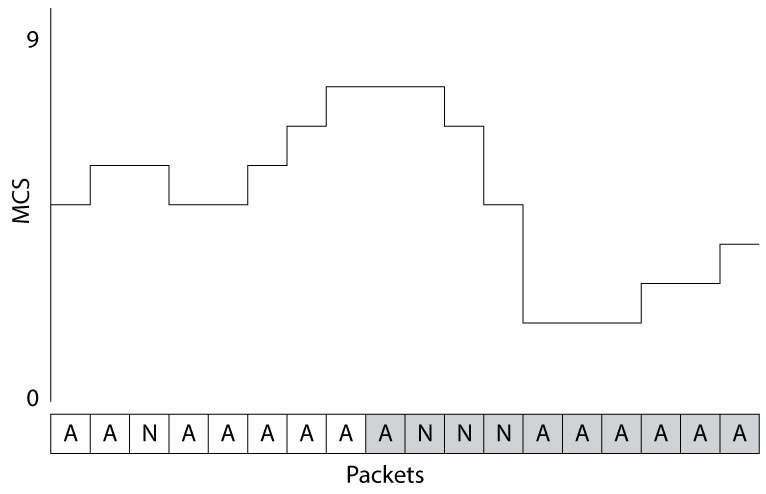
\includegraphics[width=0.6\textwidth]{bufer.jpg}
\caption{\label{fig:buffer}MCS switching with buffer NACK}
\end{figure}

The algorithm also starts at a higher MCS index for transmission. Since the paradigm of aggressive downshift is used, even if there is an error in the beginning, this is compensated for faster than if needed to upshift. The higher the bandwidth available, the higher the initial MCS index that can be used.


\section{Results and interpretation:}
In this section the results obtained from different scenarios are compared with the stock algorithm in the example from WLAN Toolbox in matlab. For the initial comparison the delay profile model was changed and tested for distances before and after the breakpoint. \Cref{fig:delayProfile} shows the result for Model F which has a breakpoint distance of 30m. \Cref{table:delayProfile} shows the result from other delay profiles. Model D shows a small decrease in performance for the new algorithm. This is because the given code was optimized for this scenario. When averaging the values of the different models, at a distance before the breakpoint there is an improvement of 2.7 Mbps and 8 \% reduction in error count. At the breakpoint distance the improvement is 2.02 Mbps in throughput and 7 \% reduction in error rate. Individually we see that in model C there is an improvement of 5.8 Mbps and a 22 \% reduction in error rate in model F.

\begin{figure}[h]
\centering
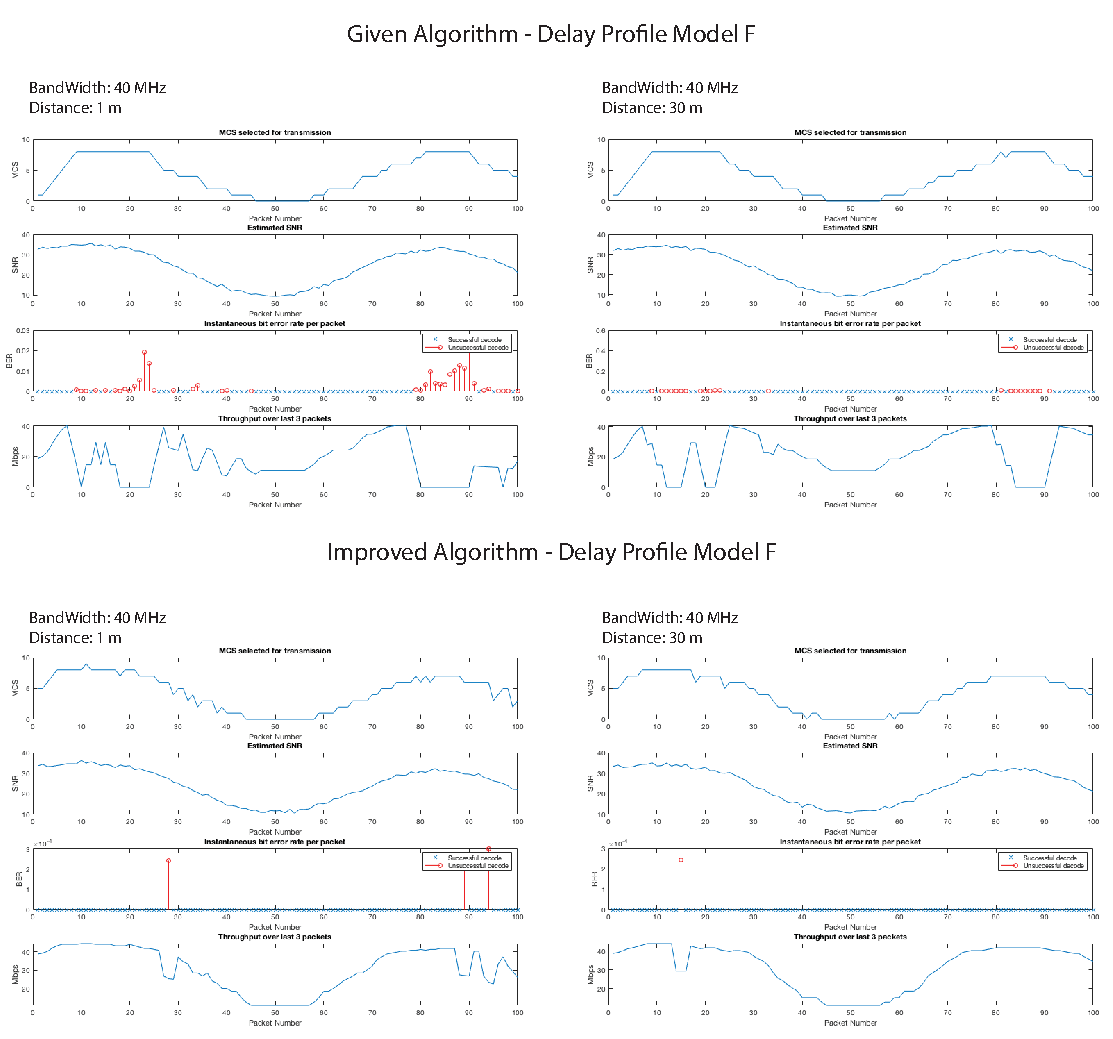
\includegraphics[width=1\textwidth]{DelayProfile.pdf}
\caption{Comparison between given and improved algorithm}
\label{fig:delayProfile}
\end{figure}


\begin{table}[h]
% Please add the following required packages to your document preamble:
% \usepackage{multirow}
\centering
\caption{\textbf{Performance Comparison for Different Delay Profile Models}}
\label{table:delayProfile}
\begin{tabular}{|l|l|l|l|}
\hline
\multicolumn{2}{|c|}{\textbf{Distance (in m)}}                                                      & \multicolumn{1}{c|}{\textbf{1}} & \multicolumn{1}{c|}{\textbf{5}} \\ \hline
\multicolumn{1}{|c|}{\multirow{2}{*}{\textbf{Model A (Given)}}} & \textbf{Throughtput}              & 24.0984                         & 17.1855                         \\ \cline{2-4}
\multicolumn{1}{|c|}{}                                          & \textbf{BER} & 0                               & 0.12                            \\ \hline
\multirow{2}{*}{\textbf{Model A (Proposed)}}                    & \textbf{Throughtput}              & 24.461                          & 22.4021                         \\ \cline{2-4}
                                                                & \textbf{BER}                      & 0                               & 0                               \\ \hline
\multirow{2}{*}{\textbf{Model B (Given)}}                       & \textbf{Throughtput}              & 23.2959                         & 24.524                          \\ \cline{2-4}
                                                                & \textbf{BER}                      & 0.09                            & 0                               \\ \hline
\multirow{2}{*}{\textbf{Model B (Proposed)}}                    & \textbf{Throughtput}              & 25.4821                         & 24.2767                         \\ \cline{2-4}
                                                                & \textbf{BER}                      & 0                               & 0                               \\ \hline
\multirow{2}{*}{\textbf{Model C(Given)}}                        & \textbf{Throughtput}              & 25.9087                         & 28.891                          \\ \cline{2-4}
                                                                & \textbf{BER}                      & 0.04                            & 0.07                            \\ \hline
\multirow{2}{*}{\textbf{Model C (Proposed)}}                    & \textbf{Throughtput}              & 31.077                          & 30.352                          \\ \cline{2-4}
                                                                & \textbf{BER}                      & 0                               & 0                               \\ \hline
\multirow{2}{*}{\textbf{Model D(Given)}}                        & \textbf{Throughtput}              & 29.2646                         & 23.3907                         \\ \cline{2-4}
                                                                & \textbf{BER}                      & 0.02                            & 0.02                            \\ \hline
\multirow{2}{*}{\textbf{Model D (Proposed)}}                    & \textbf{Throughtput}              & 25.624                          & 23.4762                         \\ \cline{2-4}
                                                                & \textbf{BER}                      & 0                               & 0.01                            \\ \hline
\multirow{2}{*}{\textbf{Model E (Given)}}                       & \textbf{Throughtput}              & 26.3504                         & 25.0963                         \\ \cline{2-4}
                                                                & \textbf{BER}                      & 0.03                            & 0.03                            \\ \hline
\multirow{2}{*}{\textbf{Model E (Proposed)}}                    & \textbf{Throughtput}              & 25.8637                         & 25.8782                         \\ \cline{2-4}
                                                                & \textbf{BER}                      & 0.01                            & 0.01                            \\ \hline
\multirow{2}{*}{\textbf{Model F (Given)}}                       & \textbf{Throughtput}              & 16.1078                         & 20.1851                         \\ \cline{2-4}
                                                                & \textbf{BER}                      & 0.39                            & 0.23                            \\ \hline
\multirow{2}{*}{\textbf{Model F (Proposed)}}                    & \textbf{Throughtput}              & 24.8002                         & 24.9964                         \\ \cline{2-4}
                                                                & \textbf{BER}                      & 0.03                            & 0.01                            \\ \hline
\end{tabular}
\end{table}



Another property that was used to check for improvements with varying channel configuration is the environmental speed. This defines the speed of the scatterers such as dust and humidity. The higher the speed, the more detrimental the effect to the signal. From \cref{table:envSpeed} ,it can be seen that the new algorithm performs better in more detrimental cases where the scatterer speed is increased.

\FloatBarrier
\begin{table}[h]
\centering
\caption{\textbf{Environmental Speed}}
\label{table:envSpeed}
\begin{tabular}{|c|l|l|l|l|}
\hline
\multicolumn{1}{|l|}{\textbf{Distance(in Km/hr)}} & \multicolumn{1}{c|}{\textbf{\begin{tabular}[c]{@{}c@{}}Throughput\\  (Given)\end{tabular}}} & \textbf{\begin{tabular}[c]{@{}l@{}}Throughput\\  (Proposed)\end{tabular}} & \multicolumn{1}{c|}{\textbf{\begin{tabular}[c]{@{}c@{}}BER \\ (Given)\end{tabular}}} & \multicolumn{1}{c|}{\textbf{\begin{tabular}[c]{@{}c@{}}BER\\ (Proposed)\end{tabular}}} \\ \hline
0.01                                              & 22.7345                     & 25.8921                        & 0.16                & 0                      \\ \hline
0.089                                             & 20.1851                     & 24.9964                        & 0.23                & 0.01                   \\ \hline
0.12                                              & 21.0176                     & 24.9446                        & 0.18                & 0.02                   \\ \hline
0.2                                               & 20.2265                     & 22.6199                        & 0.27                & 0.06                   \\ \hline
\end{tabular}
\end{table}
\FloatBarrier

The case where different waves are passed through the same medium has to be explored as well. When the waveform bandwidth is increased, the throughput should increase as well since more data can be enclosed. This will decrease the bit error rate as well. Since the new algorithm benefits from presence of NACK, the improvement from higher bandwidths are not as high as from lower bandwidths. Another property of the waveform that was tested on is the channel coding. Compared with BCC, no tail bits and padding bits are added for LDPC. Another difference is that multiple FEC (Forward Error Correction) encoders can be used in BCC. The new algorithm shows big improvements in BCC encoding while the improvement in LDPC is only seen from the bit error rate \cref{table:channelCoding}.

\FloatBarrier
\begin{table}[h]
\centering
\caption{\textbf{Channel Coding}}
\label{table:channelCoding}
\begin{tabular}{|l|l|l|l|l|}
\hline
\textbf{Coding Type} & \multicolumn{1}{c|}{\textbf{\begin{tabular}[c]{@{}c@{}}Throughput\\  (Given)\end{tabular}}} & \textbf{\begin{tabular}[c]{@{}l@{}}Throughput\\  (Proposed)\end{tabular}} & \multicolumn{1}{c|}{\textbf{\begin{tabular}[c]{@{}c@{}}BER \\ (Given)\end{tabular}}} & \multicolumn{1}{c|}{\textbf{\begin{tabular}[c]{@{}c@{}}BER\\ (Proposed)\end{tabular}}} \\ \hline
BCC                  & 20.1851                     & 24.9964                        & 0.03                 & 0.01                    \\ \hline
LDPC                 & 26.0297                     & 25.8032                        & 0.01                 & 0                       \\ \hline
\end{tabular}
\end{table}
\FloatBarrier

The next property that was tested for, is the guard interval of the transmission. To ensure non-interference from subsequent transmissions there needs to be proper guard interval in place. The greater the interval, the more immune the signal is to reflections and overlaps. \Cref{table:guardInterval} shows the improvement in throughput and bit error rate for the given and new algorithm. Here again there is significant improvement (4.8 Mbps, 22 less ber).

\FloatBarrier
\begin{table}[h]
\centering
\caption{\textbf{Guard Interval}}
\label{table:guardInterval}
\begin{tabular}{|l|l|l|l|l|}
\hline
\textbf{Guard Interval} & \multicolumn{1}{c|}{\textbf{\begin{tabular}[c]{@{}c@{}}Throughput\\  (Given)\end{tabular}}} & \textbf{\begin{tabular}[c]{@{}l@{}}Throughput\\  (Proposed)\end{tabular}} & \multicolumn{1}{c|}{\textbf{\begin{tabular}[c]{@{}c@{}}BER \\ (Given)\end{tabular}}} & \multicolumn{1}{c|}{\textbf{\begin{tabular}[c]{@{}c@{}}BER\\ (Proposed)\end{tabular}}} \\ \hline
Long                    & 20.1851                     & 24.9964                        & 0.23                 & 0.01                    \\ \hline
Short                   & 15.1496                     & 16.3096                        & 0.43                 & 0.34                    \\ \hline
\end{tabular}
\end{table}
\FloatBarrier

%\vspace*{10px}

\section{Conclusion:}
The algorithm proposed here has a clear advantage when SNR values suddenly change since multiple non-acknowledgements make the down shift more aggressive. This algorithm becomes even more efficient when used along side HARQ (hybrid automatic repeat request). The algorithm prevents multiple NACK to occur simultaneously which prevents overflowing the HARQ buffer. This also means that less retransmissions are required.

In very few scenarios such as with LDPC channel coding the throughput is slightly less than the test case but all scenarios show reduced bit error count. With increasing packet count the probability of bit error count increases, thus making the new algorithm better. From all the scenarios that were run, the best improvement achieved in throughput is 5.8 Mbps and 36\% reduction in error count.



\end{document}
